\chapter{Common Polynomial Products}

In math and physics, you will run into certain kinds of polynomials
over and over again. In this chapter, We are going to cover some
patterns that you will want to be able to recognize.

\section{Difference of squares}

Watch \textbf{Polynomial special products: difference of squares} from Khan Academy at \url{https://youtu.be/uNweU6I4Icw}.

If you are asked what $(3x - 7)(3x + 7)$ is, you would use the
distributive property to expand that to $(3x)(3x) + (3x)(7) + (-7)(3x) + (-7)(7)$.
Two of the terms cancel each other, so this is $(3x)^2 - (7)^2$. This would simplify to $9x^2 - 49$

You will see this pattern often. Anytime you see $(a + b)(a - b)$, you should immediately
recognize it equals $a^2 - b^2$. (Note that the order doesn't matter: $(a - b)(a + b)$ also $a^2 - b^2$.)

Working the other way is important too. Any time you see $a^2 - b^2$,
that you should recognize that you can change that into the product
$(a + b)(a - b)$. Making something into a product like this is known as
\emph{factoring}. You probably have done prime factorization of
numbers like $42 = 2 \times 3 \times 7$. In the next couple of
chapters, you will learn to factorize polynomials.

\begin{Exercise}[title={Difference of Squares}, label=diffsquares]
  Simplify the following products:
  \Question{$(2x - 3)(2x + 3)$}
  \Question{$(7 + 5x^3)(7 - 5x^3)$}
  \Question{$(x - a)(x + a)$}
  \Question{$(3 - \pi)(3 + \pi)$}
  \Question{$(-4x^3 + 10)(-4x^3 - 10)$}
  \Question{$(x + \sqrt{7})(x - \sqrt{7})$}
  Factor the following polynomials:
    \Question{$x^2 - 9$}
    \Question{$49 - 16x^6$}
    \Question{$\pi^2 - 25x^8$}
    \Question{$x^2 - 5$}
\end{Exercise}
\begin{Answer}[ref=diffsquares]
  $(2x - 3)(2x + 3) = 4x^2 - 9$
  
  $(7 + 5x^3)(7 - 5x^3) = 49 - 25x^6$
  
  $(x - a)(x + a) = x^2 - a^2$
  
  $(3 - \pi)(3 + \pi) = 9 - \pi^2$
  
  $(-4x^3 + 10)(-4x^3 - 10) = 16x^6 - 100$
  
  $(x + \sqrt{7})(x - \sqrt{7}) = x^2 - 7$

  $x^2 - 9 = (x + 3)(x - 3)$

  $49 - 16x^6 = (7 + 4x^3)(7 + 4^3)$
  
  $\pi^2 - 25x^8 = (\pi + 5x^4)(\pi - 5x^4)$
  
  $x^2 - 5 = (x + \sqrt{5})(x - \sqrt{5})$

\end{Answer}

We are often interested in the roots of a polynomial. That is, we want
to know ``For what values of $x$ does the polynomial evaluate to
zer?'' For example, when you deal with falling bodies, the first
question you might ask would be ``How many seconds before the hammer
hits the ground?''  Once you have factored a polynomial into
binomials, you can easily find the roots.

For example, what are the roots of $x^2 - 5$? You just factored it
into $(x + \sqrt{5})(x - \sqrt{5})$ This product is zero if and only
if one of the factors is zero. The first factor is only zero when $x$
is $-\sqrt{5}$. The second factor is zero only when $x$ is
$\sqrt{5}$. Those are the only two roots of this
polynomial.

Let's check that result. $\sqrt{5}$ is a little more than 2.2.  Using
your Python code, you can graph the polynomial:
\begin{Verbatim}
import poly.py
import matplotlib.pyplot as plt

# x**2 - 5
pn = [-5.0, 0.0, 1.0]

# These lists will hold our x and y values
x_list = []
y_list = []

# Start at x=-3
current_x =-3.0

# End at x=3.0
while current_x < 3.0:
    current_y = poly.evaluate_polynomial(pn, current_x)

    # Add x and y to respective lists
    x_list.append(current_x)
    y_list.append(current_y)

    # Move x forward
    current_x += 0.1

# Plot the curve
plt.plot(x_list, y_list)
plt.grid(True)
plt.show()
\end{Verbatim}

You should get a plot like this:
\begin{figure}[htbp]
    \centering
    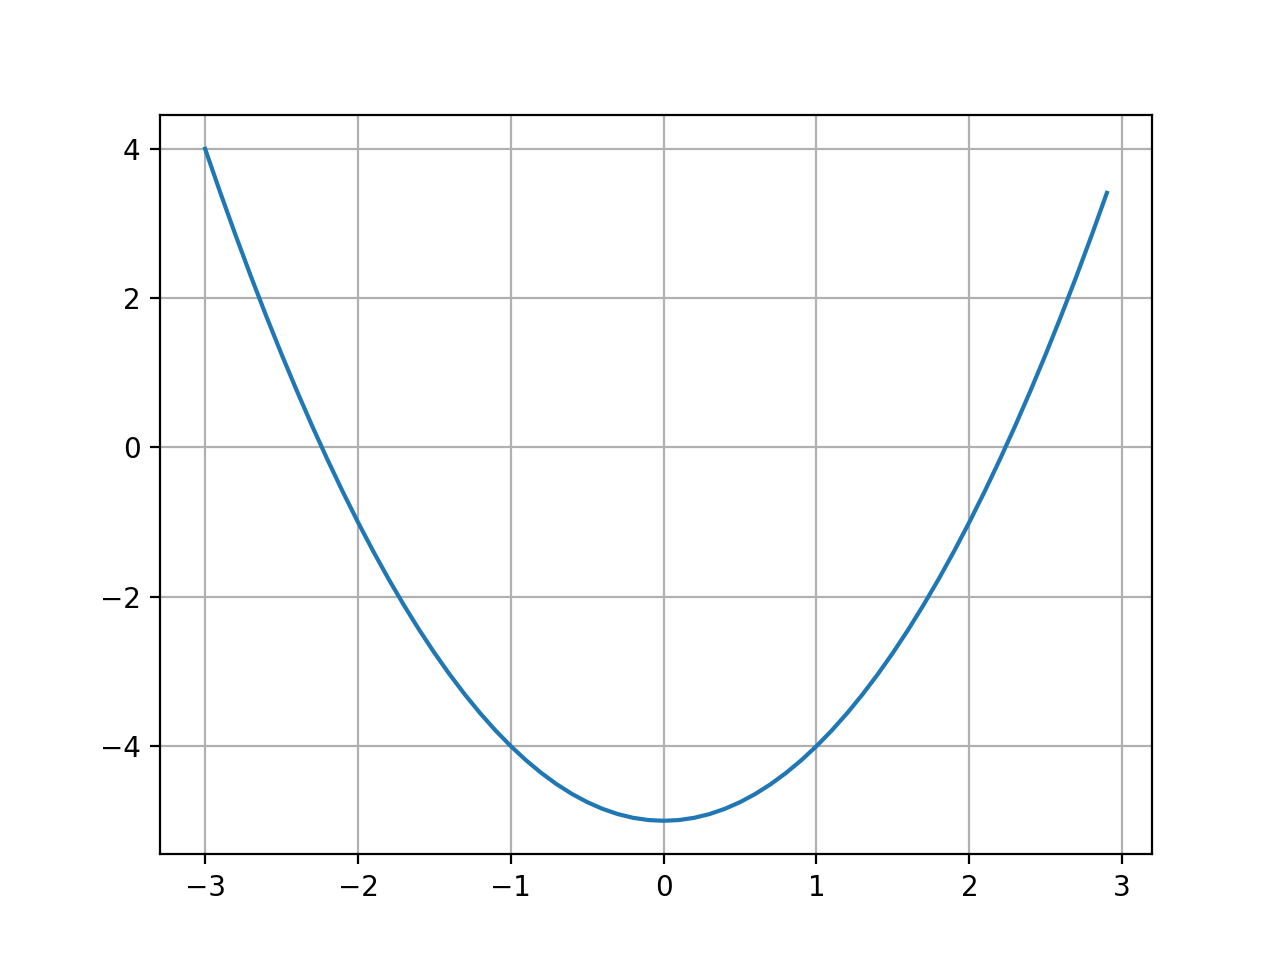
\includegraphics[width=\textwidth]{sqrt5.png}
    \caption{A graph of $x^2-5$ showing the roots on the x-axis.}
    \label{fig:sqrt5}
\end{figure}

It does, indeed, seem to cross the x-axis near -2.2 and 2.2.

\section{Powers of binomials}

You can raise whole polynomials to exponents. For example,
\begin{multline*}
  (3x^3 + 5)^2 = (3x^3 + 5)(3x^3 + 5) \\ = 9x^6 + 15x^3 + 15x^3 + 25 = 9x^6 + 30x^3 + 25 
\end{multline*}

A polynomial with two terms is called a \emph{binomial}. $5x^9 - 2x^4$,
for example, is a binomial. In this section, we are going to
develop some handy techniques for raising a binomial to some power.

Looking at the previous example, you can see that for any monomials $a$ and $b$, $(a + b)^2 = a^2 + 2ab + b^2$. This is referred to as a perfect square binomial. \index{perfect squares}
So, for example, $(7x^3 + \pi)^2 = 49x^6 + 14\pi x^3 + \pi^2$

\begin{Exercise}[title={Squaring binomials}, label=squaringbinomials]
  Simply the following
  \Question{$(x + 1)^2$}
  \Question{$(3x^5 + 5)^2$}
  \Question{$(x^3 - 1)^2$}
  \Question{$(x - \sqrt{7})^2$}
  
\end{Exercise}
\begin{Answer}[ref=squaringbinomials]
  $(x+1)^2 = x^2 + 2x + 1$

  $(3x^5 + 5)^2 = 9x^10 + 30x^5 + 25$

  $(x^3 - 1)^2 = x^6 - 2x^3 + 1$

  $(x - \sqrt{7})^2 = x^2 - 2x\sqrt{7} + 7$
\end{Answer}

What about $(x + 2)^3$? You can do it as two separate multiplications:
\begin{multline*}
  (x+2)^3 = (x+2)(x+2)(x+2) \\
  = (x + 2)(x^2 + 4x + 4) = x^3 + 4x^2 + 4x + 2x^2 + 8x + 8 \\
  = x^3 + 6x^2 + 12x + 8
\end{multline*}
In general, we can say that for any monomials $a$ and $b$, $(a + b)^3 = a^3 + 3a^2b + 3ab^2 + b^3$.

What about higher powers? $(a + b)^4$, for example? You could use the
distributive property four times, but it starts to get pretty tedious.

Here is a trick. This is known as \emph{Pascal's triangle}
\begin{equation*}
\begin{array}{c}
 1 \\
 1 \quad 1 \\
 1 \quad 2 \quad 1 \\
 1 \quad 3 \quad 3 \quad 1 \\
 1 \quad 4 \quad 6 \quad 4 \quad 1 \\
 1 \quad 5 \quad 10 \quad 10 \quad 5 \quad 1 \\
 1 \quad 6 \quad 15 \quad 20 \quad 15 \quad 6 \quad 1 \\
 1 \quad 7 \quad 21 \quad 35 \quad 35 \quad 21 \quad 7 \quad 1 \\
 \ldots
\end{array}
\end{equation*}
Each entry is the sum of the two above it.

The coefficients of each term are given by the entries in Pascal's triangle:
\begin{equation*}
(a + b)^4 = 1a^4 + 4a^3b + 6a^2 b^2 + 4 a b^3 + 1 b^4   
\end{equation*}

\begin{Exercise}[title={Using Pascal's Triangle}, label=pascalbinomial]
    \Question{What is $(x + \pi)^5$?}
\end{Exercise}
\begin{Answer}[ref=pascalbinomial]
  $(x + \pi)^5 = x^5 + 5\pi x^4 + 10\pi^2 x^3 + 10 \pi^3 + x^2 + 5 \pi^2 x + \pi^5$
\end{Answer}
